% -*- latex -*-

\chapter{Build and Install \VTKm}
\label{chap:BuildAndInstall}

Before we begin describing how to develop with \VTKm, we have a brief overview of how to build \VTKm, optionally install it on your system, and start your own programs that use \VTKm.

\section{Getting \VTKm}

\VTKm is an open source software product where the code is made freely available.
To get the latest released version of \VTKm, go to the \VTKm releases page:

\begin{quote}
  \url{http://m.vtk.org/index.php/VTK-m_Releases}
\end{quote}

For access to the most recent work, the \VTKm development team provides public anonymous read access to their main source code repository.
The main \VTKm repository on a gitlab instance hosted at Kitware, Inc.
The repository can be browsed from its project web page:

\begin{quote}
  \url{https://gitlab.kitware.com/vtk/vtk-m}
\end{quote}

\index{git|(}

The source code in the \VTKm repository is access through the \textfilename{git} version control tool.
If you have not used \textfilename{git} before, there are several resources available to help you get familiar with it.
Github has a nice setup guide (\url{https://help.github.com/articles/set-up-git}) to help you get up and running quickly.
For more complete documentation, we recommend the \emph{Pro Git} book (\url{https://git-scm.com/book}).

To get a copy of the \VTKm repository, issue a git clone command.

\begin{blankexample}{Cloning the main \VTKm git repository.}
git clone https://gitlab.kitware.com/vtk/vtk-m.git
\end{blankexample}

The git clone command will create a copy of all the source code to your local machine.
As time passes and you want to get an update of changes in the repository, you can do that with the git pull command.

\begin{blankexample}{Updating a git repository with the pull command.}
git pull
\end{blankexample}

\begin{didyouknow}
  The proceeding examples for using git are based on the \textfilename{git} command line tool, which is particularly prevalent on Unix-based and Mac systems.
  There also exist several GUI tools for accessing git repositories.
  These tools each have their own interface and they can be quite different.
  However, they all should have roughly equivalent commands named ``clone'' to download a repository given a url and ``pull'' to update an existing repository.
\end{didyouknow}

\index{git|)}


\section{Configure \VTKm}

\index{CMake|(}

\VTKm uses a cross-platform configuration tool named CMake to simplify the configuration and building across many supported platforms.
CMake is available from many package distribution systems and can also be downloaded for many platforms from \url{http://cmake.org}.

Most distributions of CMake come with a convenient GUI application (\textfilename{cmake-gui}) that allows you to browse all of the available configuration variables and run the configuration.
Many distributions also come with an alternative terminal-based version (\textfilename{ccmake}), which is helpful when accessing remote systems where creating GUI windows is difficult.

One helpful feature of CMake is that it allows you to establish a build directory separate from the source directory, and the \VTKm project requires that separation.
Thus, when you run CMake for the first time, you want to set the build directory to a new empty directory and the source to the downloaded or cloned files.
The following example shows the steps for the case where the \VTKm source is cloned from the git repository.
(If you extracted files from an archive downloaded from the \VTKm web page, the instructions are the same from the second line down.)

\begin{blankexample}{Running CMake on a cloned \VTKm repository.}
git clone https://gitlab.kitware.com/vtk/vtk-m.git
mkdir vtkm-build
cd vtkm-build
cmake-gui ../vtk-m
\end{blankexample}

\begin{figure}[htb]
  \centering
  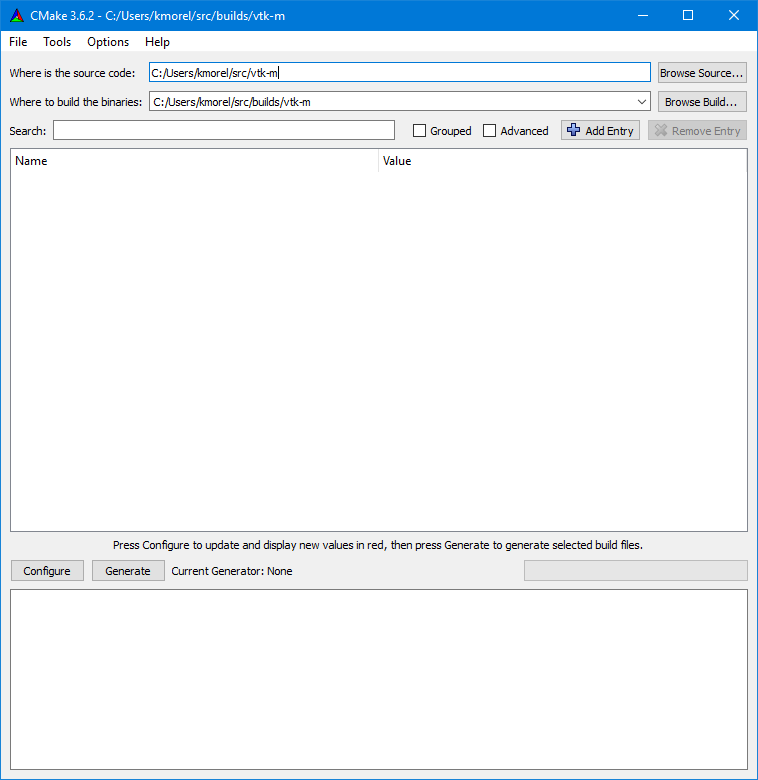
\includegraphics[width=.49\linewidth]{images/CMakeGUIBlank}
  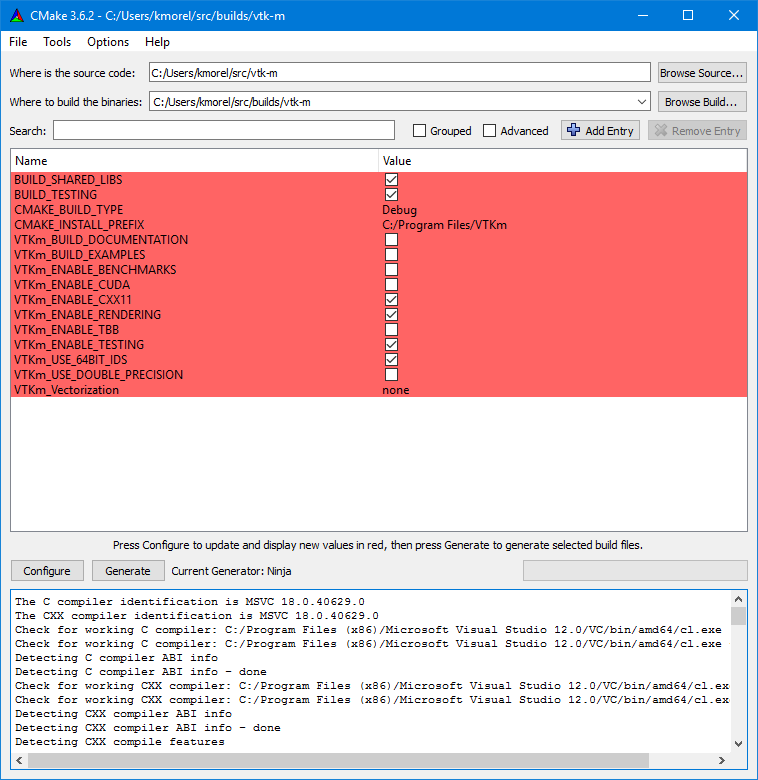
\includegraphics[width=.49\linewidth]{images/CMakeGUI}
  \caption[The CMake GUI configuring the \VTKm project.]{
    The CMake GUI configuring the \VTKm project.
    At left is the initial blank configuration.
    At right is the state after a configure pass.
  }
  \label{fig:CMakeGUI}
\end{figure}

The first time the CMake GUI runs, it initially comes up blank as shown at left in Figure~\ref{fig:CMakeGUI}.
Verify that the source and build directories are correct (located at the top of the GUI) and then click the ``Configure'' button near the bottom.
The first time you run configure, CMake brings up a dialog box asking what generator you want for the project.
This allows you to select what build system or IDE to use (e.g. make, ninja, Visual Studio).
Once you click ``Finish,'' CMake will perform its first configuration.
Don't worry if CMake gives an error about an error in this first configuration process.

\begin{commonerrors}
  Most options in CMake can be reconfigured at any time, but not the compiler and build system used.
  These must be set the first time configure is run and cannot be subsequently changed.
  If you want to change the compiler or the project file types, you will need to delete everything in the build directory and start over.
\end{commonerrors}

After the first configuration, the CMake GUI will provide several configuration options as shown in Figure~\ref{fig:CMakeGUI} on the right.
You now have a chance to modify the configuration of \VTKm, which allows you to modify both the behavior of the compiled \VTKm code as well as find components on your system.
Using the CMake GUI is usually an iterative process where you set configuration options and re-run ``Configure.''
Each time you configure, CMake might find new options, which are shown in red in the GUI.

It is often the case during this iterative configuration process that configuration errors occur.
This can occur after a new option is enabled but CMake does not automatically find the necessary libraries to make that feature possible.
For example, to enable TBB support, you may have to first enable building TBB, configure for TBB support, and then tell CMake where the TBB include directories and libraries are.

Once you have set all desired configuration variables and resolved any CMake errors, click the ``Generate'' button. This will create the build files (such as makefiles or project files depending on the generator chosen at the beginning). You can then close the CMake GUI.

There are a great number of configuration paramters available when running CMake on \VTKm.
The following list contains the most common configuration parameters.

\begin{description}
\item[\cmakevar{BUILD\_SHARED\_LIBS}]
  Determines whether static or shared libraries are built.
\item[\cmakevar{CMAKE\_BUILD\_TYPE}]
  \index{Debug} \index{Release}
  Selects groups of compiler options from catagories like Debug and Release.
  Debug builds are, obviously, easier to debug, but they run \emph{much} slower than Release builds.
  Use Release builds whenever releasing production software or doing performance tests.
\item[\cmakevar{CMAKE\_INSTALL\_PREFIX}]
  The root directory to place files when building the install target.
\item[\cmakevar{VTKm\_BUILD\_EXAMPLES}]
  The \VTKm repository comes with an \textfilename{examples} directory.
  This macro determines whether they are built.
\item[\cmakevar{VTKm\_ENABLE\_BENCHMARKS}]
  If on, the \VTKm build includes several benchmark programs.
  The benchmarks are regression tests for performance.
\item[\cmakevar{VTKm\_ENABLE\_CUDA}]
  \index{CUDA}
  Determines whether \VTKm is built to run on CUDA GPU devices.
\item[\cmakevar{VTKm\_ENABLE\_RENDERING}]
  Determines whether to build the rendering library.
\item[\cmakevar{VTKm\_ENABLE\_TBB}]
  Determines whether \VTKm is built to run on multi-core x86 devices using the Intel Threading Building Blocks library.
\item[\cmakevar{VTKm\_ENABLE\_TESTING}]
  If on, the \VTKm build includes building many test programs.
  The \VTKm source includes hundreds of regression tests to ensure quality during development.
\item[\cmakevar{VTKm\_USE\_64BIT\_IDS}]
  If on, then \VTKm will be compiled to use 64-bit integers to index arrays and other lists.
  If off, then \VTKm will use 32-bit integers.
  32-bit integers take less memory but could cause failures on larger data.
\item[\cmakevar{VTKm\_USE\_DOUBLE\_PRECISION}]
  If on, then \VTKm will use double precision (64-bit) floating point numbers for calculations where the precision type is not otherwise specified.
  If off, then single precision (32-bit) floating point numbers are used.
  Regardless of this setting, \VTKm's templates will accept either type.
\end{description}

\index{CMake|)}
